Das Ergebnis der Datenintegrationsprüfung ist die problemlose Einbindung in das bestehende Datenbankschema. Die Anbindung der Schnittstelle zur Sage Office Line erfolgt mittels DCM-Verfahren sowie die Integration der Formulare in die bestehende Benutzeroberfläche der Sage Office Line ist aufgrund des modularen Aufbaukonzepts von Sage problemlos möglich. DCM heißt "'DLL Common Method"' und ist eine von Sage geschaffene Methode um externe Schnittstellen mit der Sage Office Line zu verbinden... \textbf{Erklärung DCM + Screenshots}

Auf den Screenshots sieht man die fertige Schnittstelle...
\begin{figure}[!ht]
    \centering
    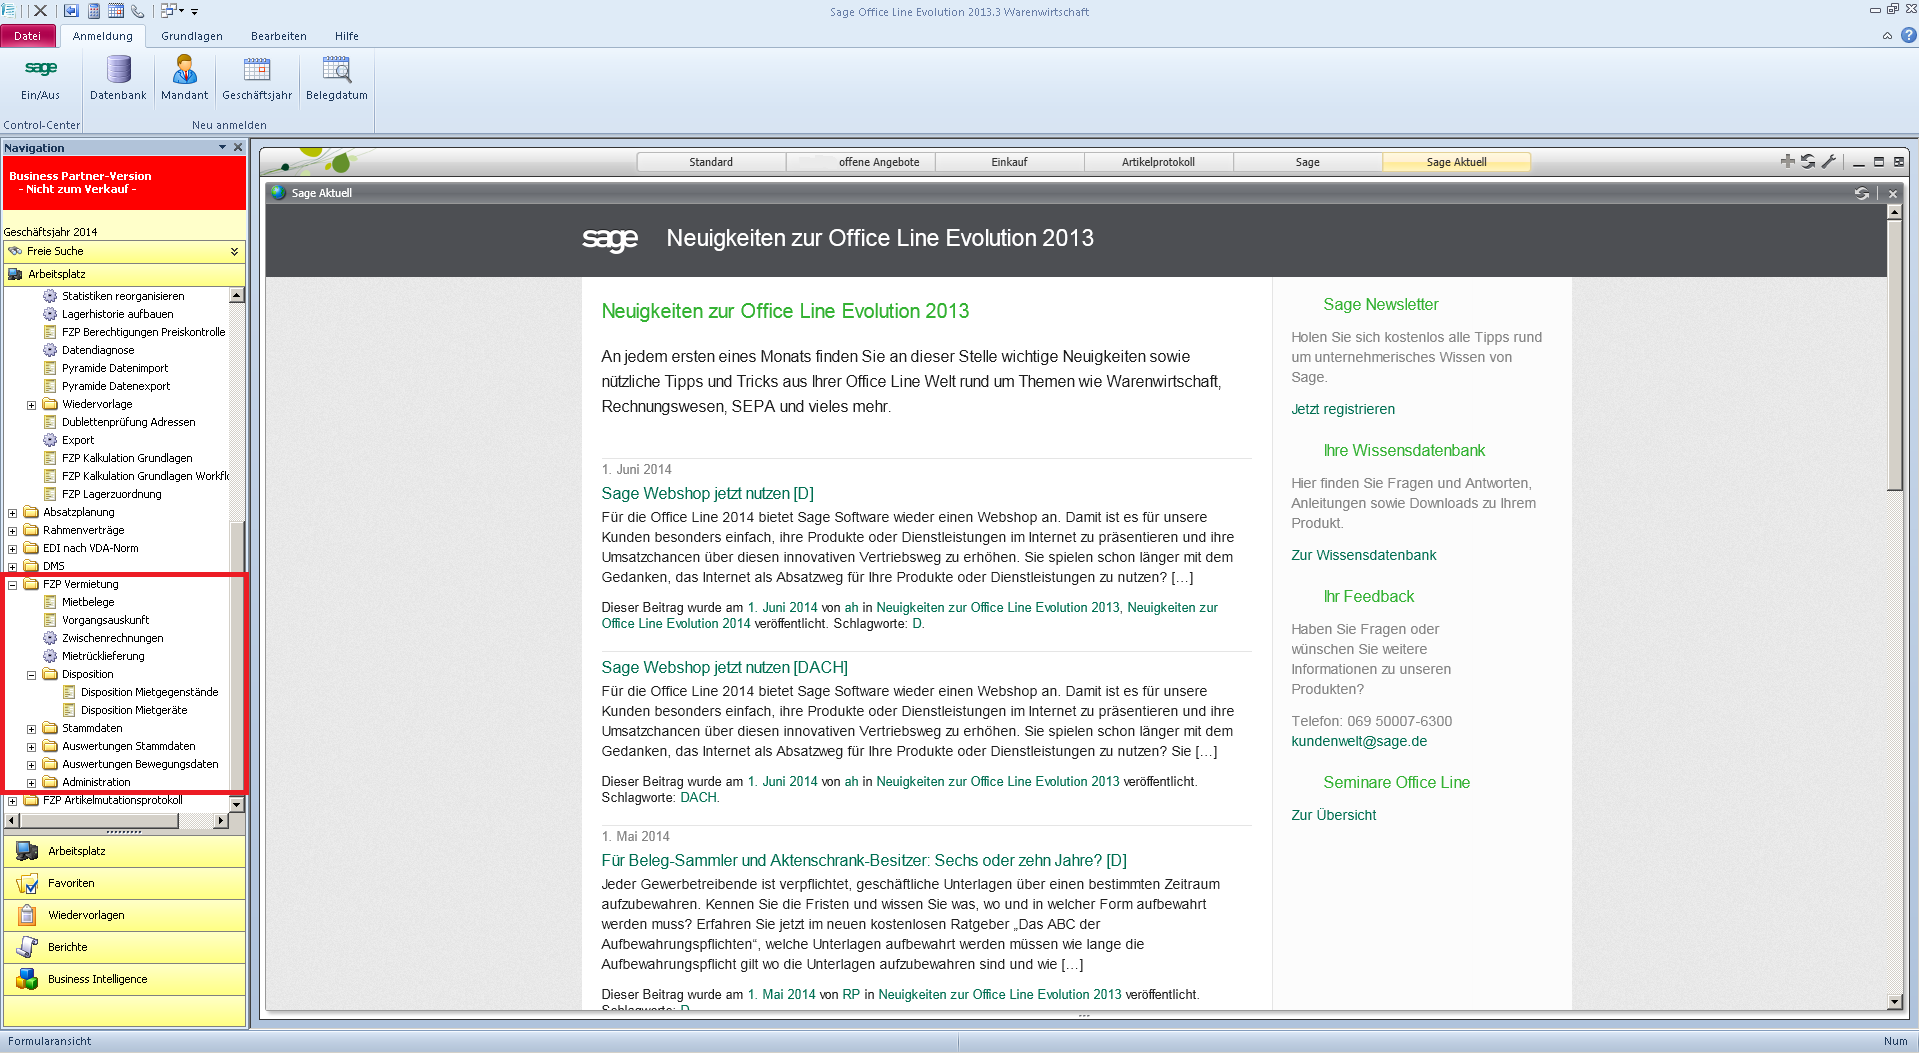
\includegraphics[height=250pt, width=450pt]{ol.PNG}
    \caption[Hauptansicht Sage Office Line]{Hauptansicht Sage Office Line}
    \label{fig:5}
\end{figure}\\
Test text
\begin{figure}[!ht]
    \centering
    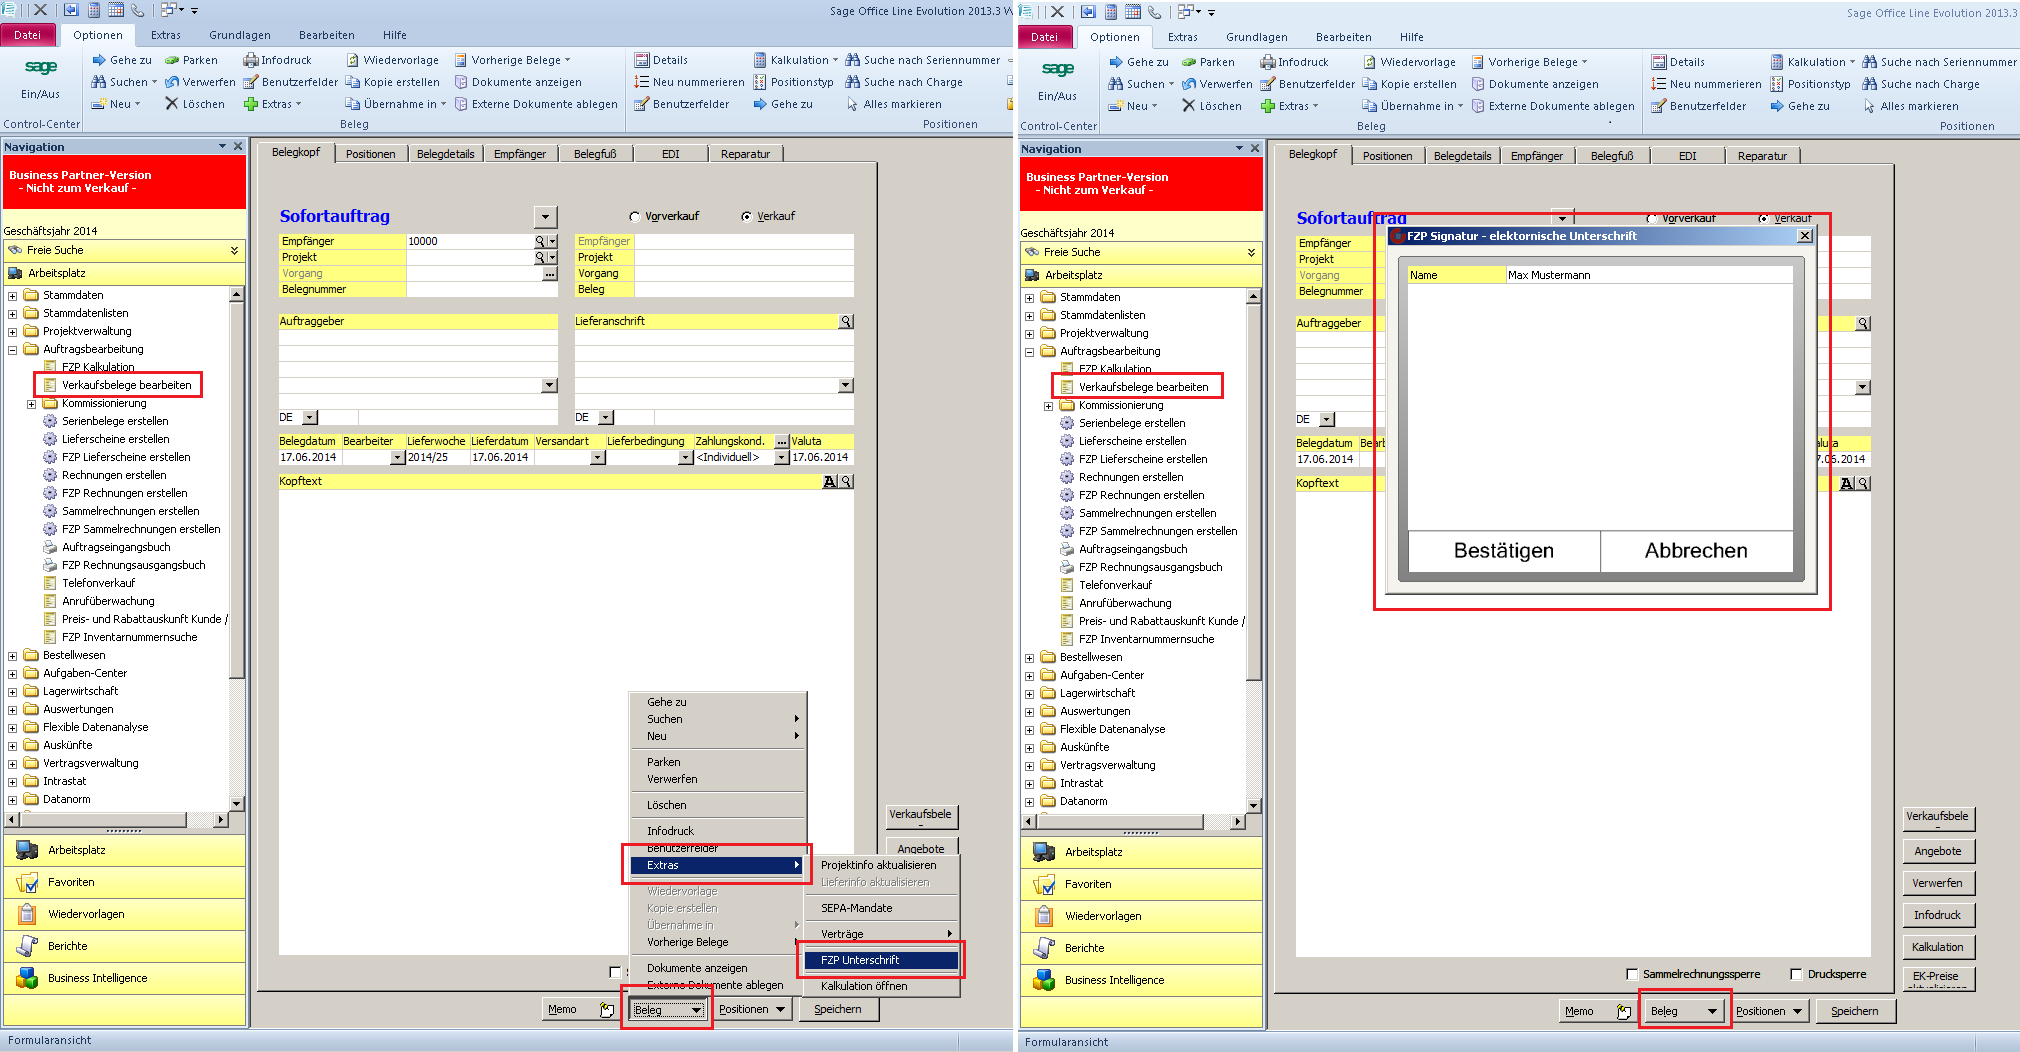
\includegraphics[height=250pt, width=450pt]{DigiSigVKBeleg3.png}
    \caption[Ablauf Erfassung digitale Signatur in Sage Office Line (Verkauf)]{Ablauf Erfassung digitale Signatur im Bereich Verkauf in Sage Office Line}
    \label{fig:6}
\end{figure}\\
Test Text 2
\begin{figure}[!ht]
    \centering
    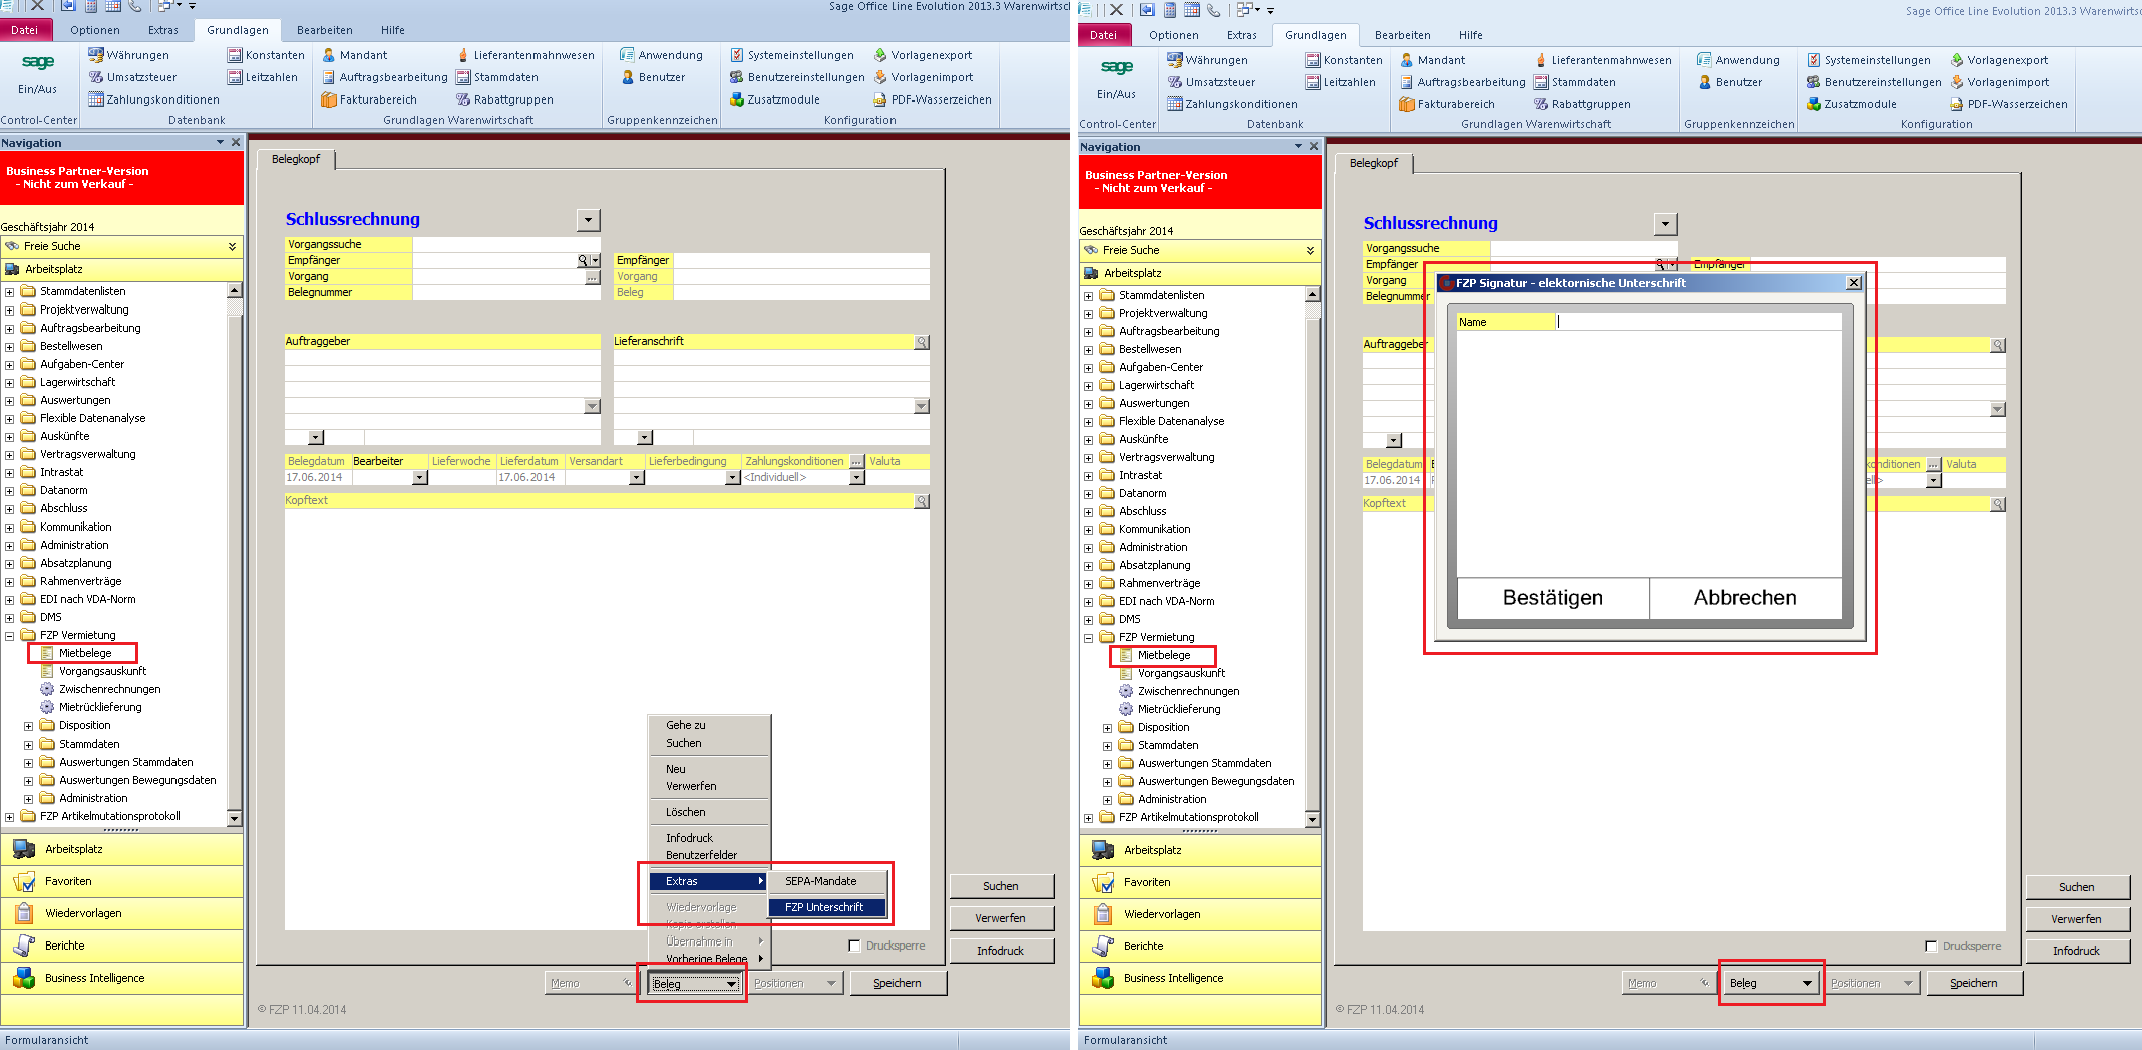
\includegraphics[height=250pt, width=450pt]{DigiSigVMBeleg3.png}
    \caption[Ablauf Erfassung digitale Signatur in Sage Office Line (Vermietung)]{Ablauf Erfassung digitale Signatur im Bereich Vermietung in Sage Office Line}
    \label{fig:7}
\end{figure}